% Section content template for individual Educative lessons
% This file contains the actual content for a specific section
% Generated from Educative API section content

% Section: Types of Databases
% Section ID: 6521598450597888
% Section Slug: types-of-databases
% Generated: 2025-12-06T21:14:18.418911

As we discussed earlier, databases are divided into two types: relational and non-relational. Let's discuss these types in detail.

\subsection{Relational databases}\label{zHzAP2aI98UMAcpQtYgL7}
\\
\textbf{Relational databases} adhere to particular schemas before storing the data. The data stored in relational databases has prior structure. Mostly, this model organizes data into one or more relations (also called tables), with a unique key for each tuple (instance). Each entity of the data consists of instances and attributes, where instances are stored in rows, and the attributes of each instance are stored in columns. Since each tuple has a unique key, a tuple in one table can be linked to a tuple in other tables by storing the primary keys in other tables, generally known as foreign keys.
\\
A Structure Query Language (SQL) is used for manipulating the database. This includes insertion, deletion, and retrieval of data.
\\
There are various reasons for the popularity and dominance of relational databases, which include simplicity, robustness, flexibility, performance, scalabilityTraditional databases are vertically scalable. Vertical scaling has limits. One might reach a point when more compute, memory, storage, or networking capability could not be added to a single node., and compatibility in managing generic data.
\\
Relational databases provide the atomicity, consistency, isolation, and durability \href{https://www.educative.io/answers/what-are-acid-properties-in-a-database}{(ACID)} properties to maintain the integrity of the database. ACID is a powerful abstraction that simplifies complex interactions with the data and hides many anomalies (like dirty reads, dirty writes, read skew, lost updates, write skew, and phantom reads) behind a simple transaction abort.
\\
But ACID is like a big hammer by design so that it's generic enough for all the problems. If some specific application only needs to deal with a few anomalies, there's a window of opportunity to use a custom solution for higher performance, though there is added complexity.
\\
Let's discuss ACID in detail:

\begin{itemize}
\item
\protect\phantomsection\label{vOe_XpK_bx79NeePaA_iw}
\textbf{Atomicity:} A transaction is considered an atomic unit. Therefore, either all the statements within a transaction will successfully execute, or none of them will execute. If a statement fails within a transaction, it should be aborted and rolled back.
\item
\protect\phantomsection\label{qVUVgUc2xCV-4EaX8sh-M}
\textbf{Consistency:} At any given time, the database should be in a consistent state, and it should remain in a consistent state after every transaction. For example, if multiple users want to view a record from the database, it should return a similar result each time.
\item
\protect\phantomsection\label{bePGv26R2sMjViT4h0-S5}
\textbf{Isolation:} In the case of multiple transactions running concurrently, they shouldn't be affected by each other. The final state of the database should be the same as the transactions that were executed sequentially.
\item
\protect\phantomsection\label{ziEKzBBzitLWOBQFXb4Nf}
\textbf{Durability:} The system should guarantee that completed transactions will survive permanently in the database even in system failure events.
\end{itemize}
\\
Various database management systems (DBMS) are used to define relational database schema along with other operations, such as storing, retrieving, and running SQL queries on data. Some of the popular DBMSs are as follows:

\begin{itemize}
\item
\protect\phantomsection\label{e3dU8wfsKYUMA18xwQx9O}
MySQL
\item
\protect\phantomsection\label{MjkiOf7eCA4HXhUHeM5c3}
Oracle Database
\item
\protect\phantomsection\label{50eUurx541gvE7I3duYye}
Microsoft SQL Server
\item
\protect\phantomsection\label{251wD8BhjUVGAo9cgBOzv}
IBM DB2
\item
\protect\phantomsection\label{4r2HEOBTxK2Qtq0qhMnap}
Postgres
\item
\protect\phantomsection\label{O5gK6T4czAXARp6Ck4CZK}
SQLite
\end{itemize}

\subsubsection{Why relational databases?}\label{B7Q-i8G69olvY1sn4sYRI}
\\
Relational databases are the default choice of software professionals for structured data storage. There are a number of advantages to these databases. One of the greatest powers of the relational database is its abstractions of ACID transactions and related programming semantics. This makes it very convenient for the end programmer to use a relational database. Let 's revisit some important features of relational databases:
\\
\paragraph{Flexibility}\label{lst3TFxD9P-fAEX5WRRHl}
\\
In the context of SQL, \textbf{data definition language (DDL)} DDL is a computer language used to create and modify the structure of database objects in a database. provides us the flexibility to modify the database, including tables, columns, renaming the tables, and other changes. DDL even allows us to modify schema while other queries are happening and the database server is running.
\\
\paragraph{Reduced redundancy}\label{BkSogF_jlmqBzxzPP6GJg}
\\
One of the biggest advantages of the relational database is that it eliminates data redundancy. The information related to a specific entity appears in one table while the relevant data to that specific entity appears in the other tables linked through foreign keys. This process is called normalization and has the additional benefit of removing an inconsistent dependencyInconsistent dependencies arise when a user searches for some data in the irrelevant table or the data is missing in the relevant table. For example, to find the customer's address it should be searched in the customer table instead of the product table..
\\
\paragraph{Concurrency}\label{N3hTg5SHZoQB8wB7HchJ5}
\\
Concurrency is an important factor while designing an enterprise database. In such a case, the data is read and written by many users at the same time. We need to coordinate such interactions to avoid inconsistency in data---for example, the double booking of hotel rooms. Concurrency in a relational database is handled through transactional access to the data. As explained earlier, a transaction is considered an atomic operation, so it also works in error handling to either roll back or commit a transaction on successful execution.
\\
\paragraph{Integration}\label{ytS52eh63-CwKTbUjfCyJ}
\\
The process of aggregating data from multiple sources is a common practice in enterprise applications. A common way to perform this aggregation is to integrate a shared database where multiple applications store their data. This way, all the applications can easily access each other's data while the concurrency control measures handle the access of multiple applications.
\\
\paragraph{Backup and disaster recovery}\label{z6VTjnZ4t3LxBg0ONPAoP}
\\
Relational databases guarantee the state of data is consistent at any time. The export and import operations make backup and restoration easier. Most cloud-based relational databases perform continuous mirroring to avoid loss of data and make the restoration process easier and quicker.

\subsubsection{Drawback}\label{dG5mnPzUitOjrxbERlsVJ}
\\
\paragraph{Impedance mismatch}\label{Zb5XC3aMlK_8N3zkVxKqb}
\\
\textbf{Impedance mismatch} is the difference between the relational model and the in-memory data structures. The relational model organizes data into a tabular structure with relations and tuples. SQL operation on this structured data yields relations aligned with relational algebra. However, it has some limitations. In particular, the values in a table take simple values that can't be a structure or a list. The case is different for in-memory, where a complex data structure can be stored. To make the complex structures compatible with the relations, we would need a translation of the data in light of relational algebra. So, the impedance mismatch requires translation between two representations, as denoted in the following figure:

\begin{figure}[htbp]
 \centering
 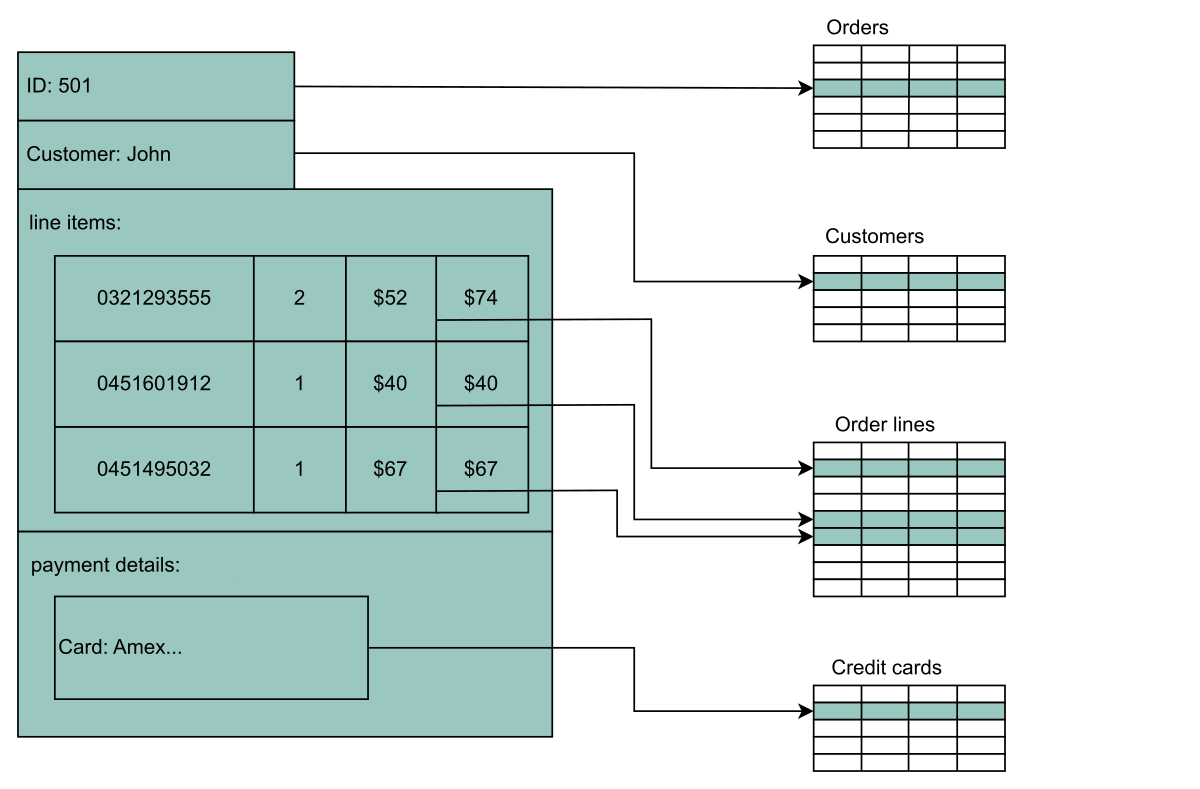
\includegraphics[width=0.5\textwidth]{Images/chapter_9/section_6521598450597888/6025220716756992.png}
 \caption{A single aggregated value in the view is composed of several rows and tables in the relational database}
\end{figure}

\subsection{Why non-relational (NoSQL) databases?}\label{ViN9oWNVQA4LngWhraPPL}
\\
A NoSQL database is designed for a variety of data models to access and manage data. There are various types of NoSQL databases, which we'll explain in the next section. These databases are used in applications that require a large volume of semi-structured and unstructured dataThe schema of the data is not known at the time of writing the data. Schema is usually defined at the time of reading such data., low latency, and flexible data models. This can be achieved by relaxing some of the data consistency restrictions of other databases. The following are some characteristics of the NoSQL database:

\begin{itemize}
\item
\protect\phantomsection\label{euoOM-xGj0tcRbAKsxpkc}
\textbf{Simple design:} Unlike relational databases, NoSQL doesn't require dealing with the impedance mismatch---for example, storing all the employees' data in one document instead of multiple tables that require join operations. This strategy makes it simple and easier to write less code, debug, and maintain.
\item
\protect\phantomsection\label{LfAhYWYZ0ST-0ZrOvaSTM}
\textbf{Horizontal scaling:} Primarily, NoSQL is preferred due to its ability to run databases on a large cluster. This solves the problem when the number of concurrent users increases. NoSQL makes it easier to scale out since the data related to a specific employee is stored in one document instead of multiple tables over nodes. NoSQL databases often spread data across multiple nodes and balance data and queries across nodes automatically. In case of a node failure, it can be transparently replaced without any application disruption.
\item
\protect\phantomsection\label{Cgi7e6baNpp01i-HdcVAF}
\textbf{Availability:} To enhance the availability of data, node replacement can be performed without application downtime. Most of the non-relational databases' variants support data replication to ensure high availability and disaster recovery.
\item
\protect\phantomsection\label{5qKVoWLop1GtavJirx0Dx}
\textbf{Support for unstructured and semi-structured data:} Many NoSQL databases work with data that doesn't have a schema at the time of database configuration or data writes. For example, document databases are structureless; they allow documents (JSON, XML, BSON, and so on) to have different fields. For example, one JSON document can have fewer fields than the other.
\item
\protect\phantomsection\label{MNdcY7dc_yzZ2P9SgmGnI}
\textbf{Cost:} Licenses for many RDBMSs are pretty expensive, while many NoSQL databases are open source and freely available. Similarly, some RDBMSs rely on costly proprietary hardware and storage systems, while NoSQL databases usually use clusters of cheap commodity servers.
\end{itemize}
\\
NoSQL databases are divided into various categories based on the nature of the operations and features, including document store, columnar database, key-value store, and graph database. We 'll discuss each of them along with their use cases from the system design perspective in the following sections.

\subsubsection{Types of NoSQL databases}\label{3bxf79GbFEb6yl2IO2V20}
\\
Various types of NoSQL databases are described below:

\begin{figure}[htbp]
 \centering
 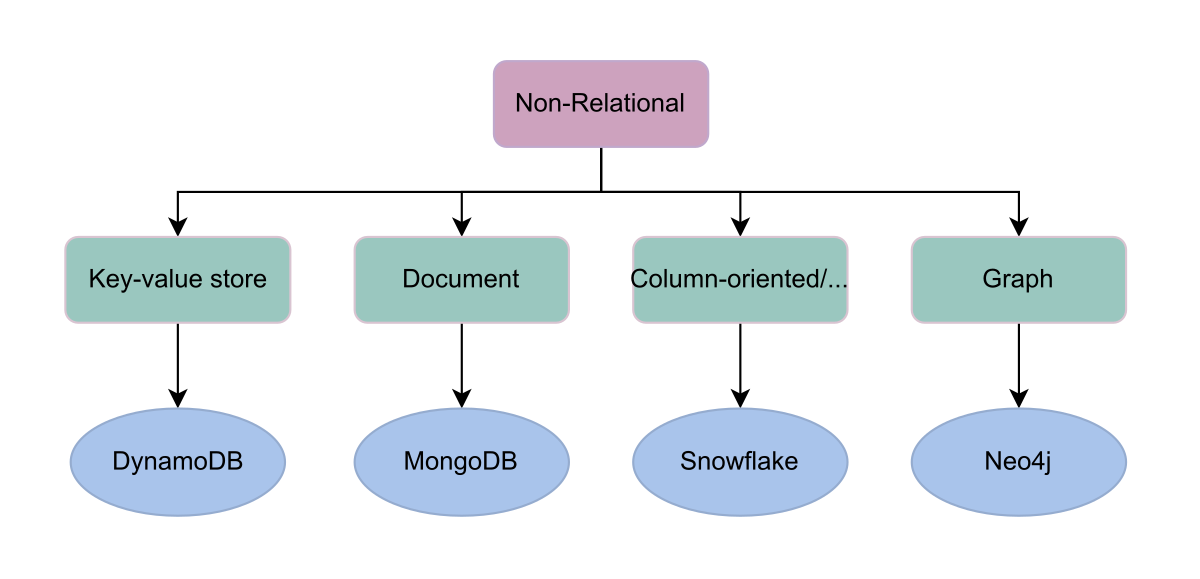
\includegraphics[width=0.5\textwidth]{Images/chapter_9/section_6521598450597888/5345427179044864.png}
 \caption{The types of NoSQL databases}
\end{figure}

\paragraph{Key-value database}\label{eHaVnbvRA_SmEN7brfS2M}
\\
\textbf{Key-value databases} use key-value methods like hash tables to store data in key-value pairs. We can see this depicted in the figure a couple of paragraphs below. Here, the key serves as a unique or primary key, and the values can be anything ranging from simple scalar values to complex objects. These databases allow easy partitioning and horizontal scaling of the data. Some popular key-value databases include Amazon DynamoDB, Redis, and Memcached DB.
\\
\textbf{Use case}: Key-value databases are efficient for session-oriented applications. Session-oriented applications, such as web applications, store users' data in the main memory or in a database during a session. This data may include user profile information, recommendations, targeted promotions, discounts, and more. A unique ID (a key) is assigned to each user's session for easy access and storage. Therefore, a better choice to store such data is the key-value database.
\\
The following figure shows an example of a key-value database. The Product\ ID and \texttt{Type} of the item are collectively considered as the primary key. This is considered as a key for this key-value database. Moreover
, the schema for storing the item attributes is defined based on the nature of the item and the number of attributes it possesses.

\begin{figure}[htbp]
 \centering
 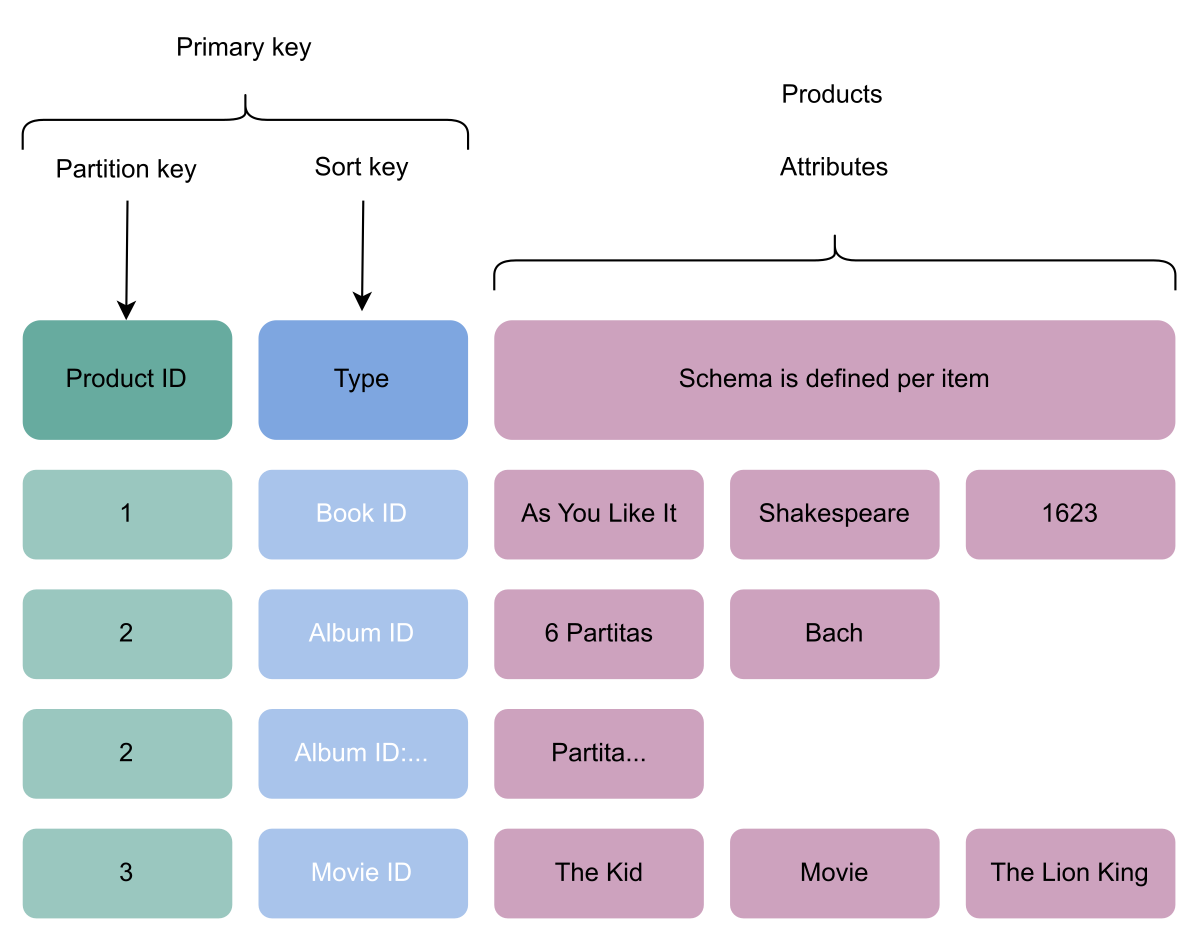
\includegraphics[width=0.5\textwidth]{Images/chapter_9/section_6521598450597888/5123805110599680.png}
 \caption{Data stored in the form of key-value pair in DynamoDB, where the key is the combination of two attributes (Product ID and Type)}
\end{figure}

\paragraph{Document database}\label{El9Tuq5s7GuhIj3kySbjQ}
\\
A \textbf{document database} is designed to store and retrieve documents in formats like XML, JSON, BSON, and so on. These documents are composed of a hierarchical tree data structure that can include maps, collections, and scalar values. Documents in this type of database may have varying structures and data. MongoDB and Google Cloud Firestore are examples of document databases.
\\
\textbf{Use case}: Document databases are suitable for unstructured catalog data, like JSON files or other complex structured hierarchical data. For example, in e-commerce applications, a product has thousands of attributes, which is unfeasible to store in a relational database due to its impact on the reading performance. Here comes the role of a document database, which can efficiently store each attribute in a single file for easy management and faster reading speed. Moreover, it's also a good option for content management applications, such as blogs and video platforms. An entity required for the application is stored as a single document in such applications.
\\
The following example shows data stored in a JSON document. This data is about a person. Various attributes are stored in the file, including \texttt{id}, \texttt{name}, \texttt{email}, and so on.

\textbf{A JSON file containing data of a businessman}

\begin{lstlisting}[language=XML]
{  "id": 1001,
	"name": "Brown",
	"title": "Mr.",
	"email": "brown@anyEmail.com",
	"cell": "123-465-9999",
	"likes": [
	"designing",
	"cycling",
	"skiing"],
	"businesses": [
	{ "name": "ABC co.",
		"partner": "Vike",
		"status": "Bankrupt",
		"date_founded": {
			"$date": "2021-12-10" } }]}
\end{lstlisting}

\paragraph{Graph database}\label{4G7f_OKlVMgtxhwG62-eR}
\\
\textbf{Graph databases} use the graph data structure to store data, where nodes represent entities, and edges show relationships between entities. The organization of nodes based on relationships leads to interesting patterns between the nodes. This database allows us to store the data once and then interpret it differently based on relationships. Popular graph databases include Neo4J, OrientDB, and InfiniteGraph. Graph data is kept in store files for persistent storage. Each of the files contains data for a specific part of the graph, such as nodes, links, properties, and so on.
\\
In the following figure, some data is stored using a graph data structure in nodes connected to each other via edges representing relationships between nodes. Each node has some properties, like \texttt{Name}, \texttt{ID}, and \texttt{Age}. The node having ID:\ 2 has the \texttt{Name} of \texttt{James} and \texttt{Age} of \texttt{29} years.

\begin{figure}[htbp]
 \centering
 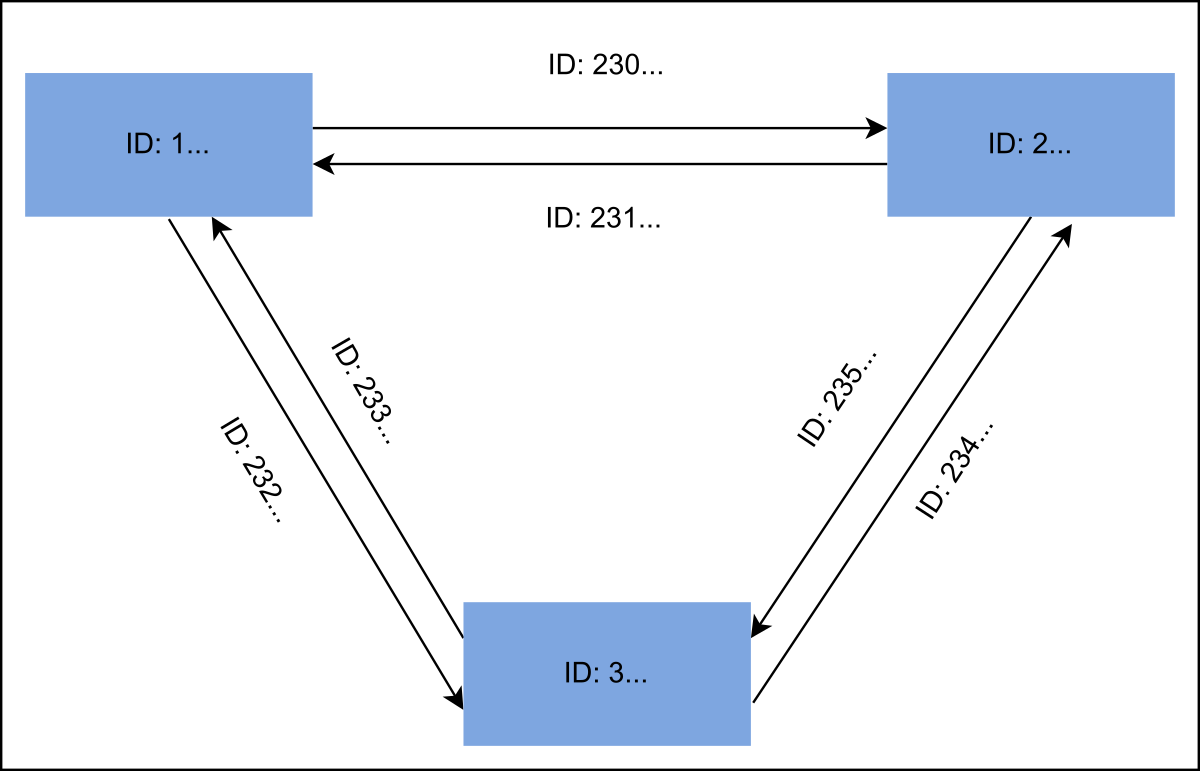
\includegraphics[width=0.5\textwidth]{Images/chapter_9/section_6521598450597888/5524191910821888.png}
 \caption{A graph consists of nodes and links. This graph captures entities and their relationships with each other}
\end{figure}

\textbf{Use case}: Graph databases can be used in social applications and provide interesting facts and figures among different kinds of users and their activities. The focus of graph databases is to store data and pave the way to drive analyses and decisions based on relationships between entities. The nature of graph databases makes them suitable for various applications, such as data regulation and privacy, machine learning research, financial services-based applications, and many more.
\\
\paragraph{Columnar database}\label{3DwyydWrIb33L8BdaC1g5}
\\
\textbf{Columnar databases} organize data by columns instead of rows. This design makes it much faster and more efficient to retrieve specific fields, especially useful when running analytics or summarizing large datasets. As a result, they are well-suited for systems where data is read frequently but updated less often. Popular columnar databases include Amazon Redshift and Google BigQuery, all widely used for high-performance analytics and data warehousing.
\\
\textbf{Use case:} These databases shine in analytical tasks that involve processing large amounts of data, such as aggregations or trend analysis. For example, in financial systems that need to calculate total transaction amounts over time, a columnar database can quickly pull just the ``amount'' field without loading unrelated data like customer names or dates.
\begin{quote}
\textbf{Note:} Another type of database often mistaken for columnar databases is the wide-column database. While columnar databases store each column's data together on disk to accelerate analytical queries and aggregations, wide-column databases, such as Apache Cassandra and HBase which organize data in rows grouped into column families, making them more suitable for write-heavy workloads and flexible, semi-structured data use cases.
\end{quote}
\\
The following figure shows an example of a columnar database, where data is stored in a column-oriented format. This is unlike relational databases, which store data in a row-oriented fashion:

\begin{figure}[htbp]
 \centering
 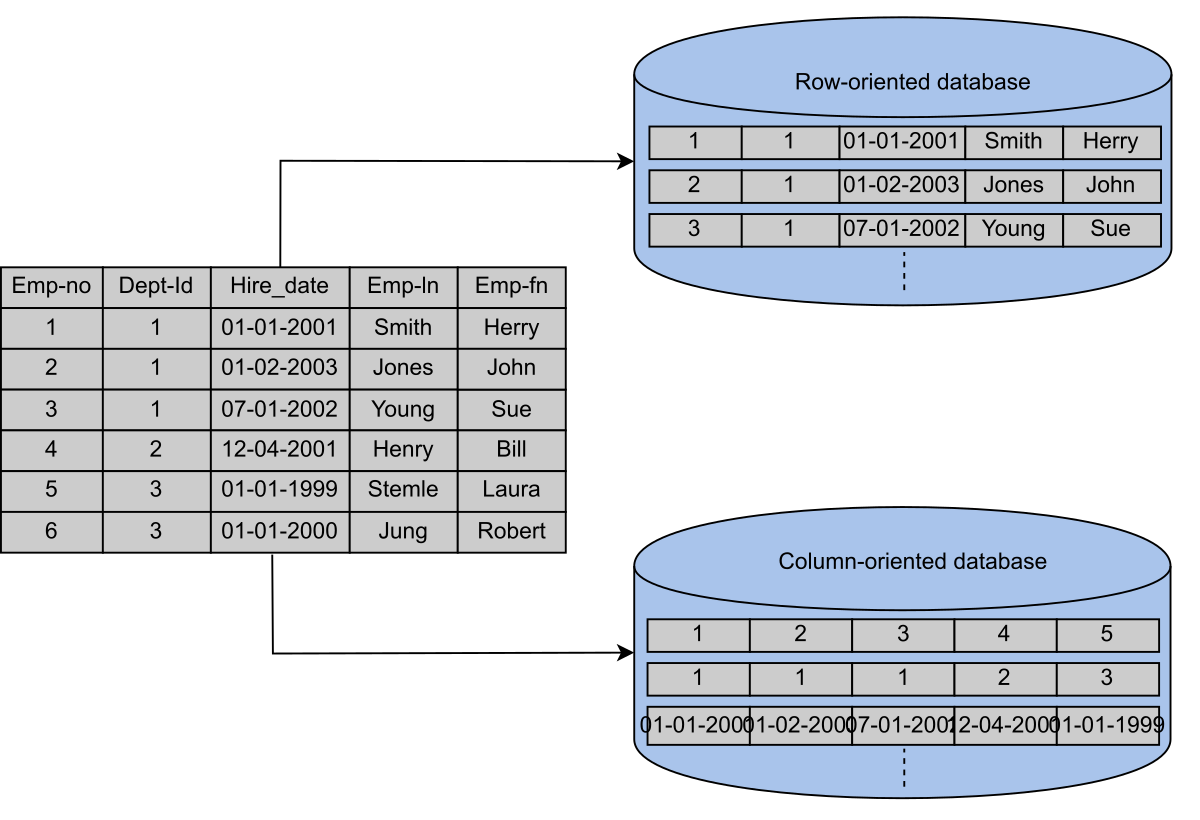
\includegraphics[width=0.5\textwidth]{Images/chapter_9/section_6521598450597888/4982612905164800.png}
 \caption{Column-oriented and row-oriented database}
\end{figure}

\subsubsection{Drawbacks of NoSQL databases}\label{f5VM78oLXjPdcW080MrBk}
\\
\paragraph{Lack of standardization}\label{w_woB3n6ehcb-jA7M1LwZ}
\\
NoSQL doesn't follow any specific standard, like how relational databases follow relational algebra. Porting applications from one type of NoSQL database to another might be a challenge.
\\
\paragraph{Consistency}\label{UN7D7jE-Qlx-6pi3XdtOw}
\\
NoSQL databases provide different products based on the specific trade-offs between consistency and availability when failures can happen. We won't have strong data integrity, like primary and referential integrities in a relational database. Data might not be strongly consistent but slowly converging using a weak model like eventual consistency.
\\
Let's assess our understanding of the lesson's content with the following question.
\\
Imagine we're designing a recommendation engine for a social networking platform with millions of users. The goal is to provide personalized recommendations for users to connect with others based on their interests, activities, and connections. Which database would be a natural fit for modeling and querying the complex relationship in a social network and why?

Provide your answer in the following interactive widget:

\textbf{Question:}

Database for personalized recommendations

\textbf{Reference Answer:}

For crafting a recommendation engine in the context of a social networking platform with millions of users, a Graph Database stands out as the ideal choice. Graph databases are purpose-built for efficiently modeling and querying complex relationships, which is inherent in a social network environment. The interconnected nature of users, interests, activities, and connections is effectively represented using nodes and edges in a graph structure. This database type excels at traversing relationships, allowing for quick and meaningful retrieval of information essential for personalized recommendations. Graph databases, with their flexibility in handling dynamic schemas and scalability for large datasets, provide a robust foundation for crafting a recommendation engine that not only considers users' interests and activities but also takes into account the intricate web of connections within the social network, leading to more accurate and relevant suggestions for connecting users.

\subsection{Choose the right database}\label{osJry6Ig2iAOetGpEijOG}
\\
Various factors affect the choice of database to be used in an application. A comparison between the relational and non-relational databases is shown in the following table to help us choose:

\textbf{Relational and Non-relational Databases}

\begin{table}[htbp]
\centering
\small
\adjustbox{max width=\textwidth}{
\begin{tabular}{|p{0.475\textwidth}|p{0.475\textwidth}|}
\hline
\textbf{Relational Database} & \textbf{Non-relational Database} \\
\hline
\hline
If the data to be stored is structured & If the data to be stored is unstructured \\
\hline
If ACID properties are required & If there's a need to serialize and deserialize data \\
\hline
If the size of the data is relatively small and can fit on a node) & If the size of the data to be stored is large \\
\hline
\end{tabular}
}
\caption{Relational and Non-relational Databases}
\end{table}

\begin{quote}
\textbf{Note}: When NoSQL databases first came into being, they were drastically different to program and use as compared to traditional databases. Though, due to extensive research in academia and industry over the last many years, the programmer-facing differences between NoSQL and traditional stores are blurring. We might be using the same SQL constructs to talk to a NoSQL store and get a similar level of performance and consistency as a traditional store. Google's Cloud SpannerSpanner: Google's Globally-Distributed Database, Google, Inc. is one such database that's geo-replicated with automatic horizontal sharding ability and high-speed global snapshots of data.
\end{quote}
\subsection{Quiz}\label{ZVoAUOSQnF_jx2rvyNesm}
\\
Test your knowledge of the different types of databases via a quiz.

\subsection*{Quiz}
\vspace{0.3cm}
\noindent
\textbf{Question 1:} Which database should we use when we have unstructured data and there's a need for high performance?
\\[0.2cm]
\begin{itemize}
 \item \textbf{[CORRECT]} MongoDB
\\[0.1cm]
\textit{Explanation:} 
MongoDB is a database that stores unstructured data and provides high performance in data-relevant operations.
 \item MySQL
 \item Oracle
\end{itemize}
\vspace{0.3cm}
\noindent
\textbf{Question 2:} When should we avoid choosing a relational database for our application?
\\[0.2cm]
\begin{itemize}
 \item \textbf{[CORRECT]} When we write an application that expects to handle a large number of read-write operations and concurrent users, but strong consistency is not required
\\[0.1cm]
\textit{Explanation:} 
When strong consistency is not required, and there are many read-write operations and concurrent users, a better choice is to use a NoSQL database. Hence , this is the right option to avoid the relational database.
 \item When we write a financial application, like a stock trading application, and we need our data to be consistent at all times
 \item When we write an application to store a lot of complex structured data
\end{itemize}
\vspace{0.3cm}
\noindent
\textbf{Question 3:} What kind of database should we use if we make a retail store application that requires storing the data in tabular format?
\\[0.2cm]
\begin{itemize}
 \item \textbf{[CORRECT]} Relational database
\\[0.1cm]
\textit{Explanation:} 
Storing tabular data means we have structured data to store; hence, a relational database is a right choice.
 \item Non-relational database
\end{itemize}
\vspace{0.3cm}
\noindent
\textbf{Question 4:} Which kind of database should we use for making an application like Facebook?
\\[0.2cm]
\begin{itemize}
 \item Relational database
 \item Non-relational database
 \item \textbf{[CORRECT]} Both
\\[0.1cm]
\textit{Explanation:} 
Facebook (and similar large-scale applications) use both SQL and NoSQL databases---SQL for structured, relational data and NoSQL for unstructured or high-volume data.
\end{itemize}
\vspace{0.3cm}
\noindent
\textbf{Question 5:} \textbf{(Select all that apply.)} We should use a document-oriented database for which applications?
\\
\textit{(Select all that apply.)}
\\[0.2cm]
\begin{itemize}
 \item \textbf{[CORRECT]} Web-based multiplayer games
\\[0.1cm]
\textit{Explanation:} 
These games handle complex objects like players or items that fit naturally into a nested document structure, which document databases store efficiently.
 \item Banking application requiring consistency
 \item Social network application, like Facebook, containing complex relationships
 \item \textbf{[CORRECT]} Real-time feeds
\\[0.1cm]
\textit{Explanation:} 
The real-time feed contains variably structured data (one feed can have different components than the others) for which a document database is a suitable option.
\end{itemize}
\vspace{0.3cm}
\noindent
\textbf{Question 6:} \textbf{(Select all that apply.)} We should use a key-value database for which scenarios?
\\
\textit{(Select all that apply.)}
\\[0.2cm]
\begin{itemize}
 \item When we create a social network like Facebook with a lot of complex relationships
\\[0.1cm]
\textit{Explanation:} 
A graph database is a suitable option to store a social network with many complex relationships.
 \item \textbf{[CORRECT]} When we need to persist user state in our application
\\[0.1cm]
\textit{Explanation:} 
User states are stored using a key-value database. A user ID can be considered key, and states can be assumed as values.
 \item \textbf{[CORRECT]} When we implement caching in our application
\\[0.1cm]
\textit{Explanation:} 
A cache like Memcached and Redis are key-value stores used for caching in different use-cases.
\end{itemize}



% End of section content